\documentclass{article}
\usepackage[letterpaper,margin=1.778cm]{geometry}
\usepackage{fancyhdr}
\usepackage{lastpage}
\usepackage{listings}
\usepackage{fancyvrb}
\usepackage{tcolorbox}
\usepackage[parfill]{parskip}
\usepackage{xstring}
\usepackage{enumitem}

\pagestyle{fancy}
\fancyhf{}
\lfoot{\StrSubstitute{\jobname}{\detokenize{_}}{ }}
\rfoot{Page \thepage\ of \pageref{LastPage}}
\renewcommand{\headrulewidth}{0pt}

\newcounter{num}

\begin{document}
\large

{\Large \bf \StrSubstitute{\jobname}{\detokenize{_}}{ }}

First, go into the folder of the period in which you are grading and click on the program {\em student\_grader.jar}. When you do this the first of two windows will open up:

\begin{center}
   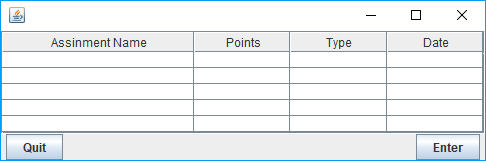
\includegraphics[scale=0.5]{startup1.png}
\end{center}

This is where you input the information about the assignments [up to 5]. The first two columns are the assignment name and total points which the teacher will give you. The third column is the assignment type which will either be {\em Work} or {\em Assessment}. {\bf It is very important that Work and Assessment is spelled correctly with the first letter being capitalized and the remaining letters be lower case.} The last column is for the assignment data and it must be in the format MM/DD/YYYY. {\bf It is very important that the month and day are written in two digits and the year is written as 4 digits. If the month or day is less than 10 add a zero to the begging of it.} Here is a sample:

\begin{center}
   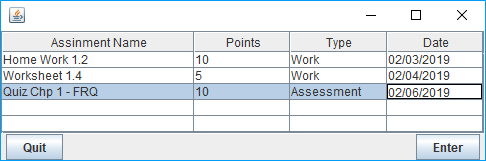
\includegraphics[scale=0.5]{startup2.png}
\end{center}

After you hit enter a new window will pop up where you can input the students' scores for each assignment. After you are done hit enter. Here is what this window looks like:

\begin{center}
    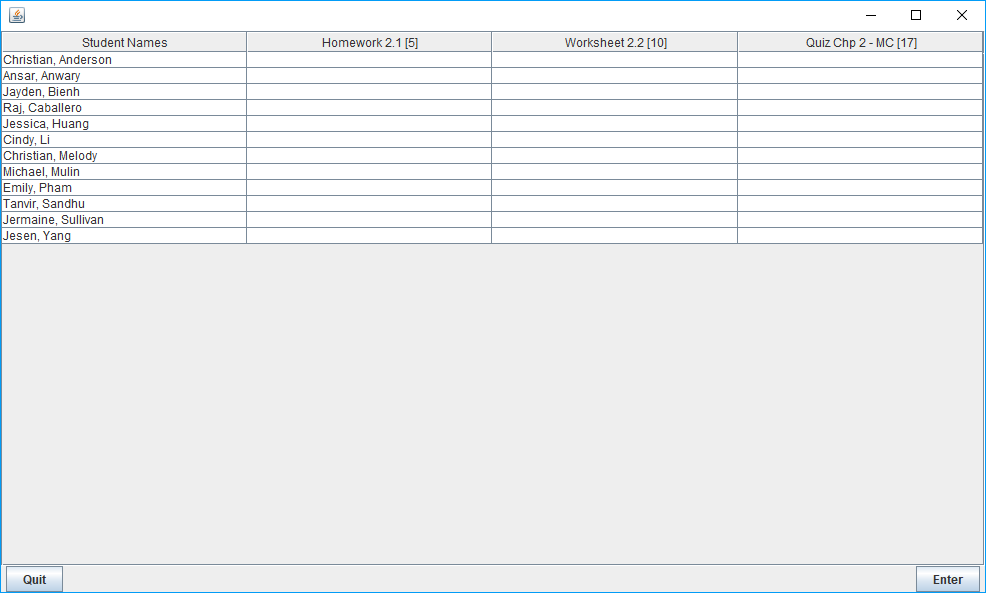
\includegraphics[scale=0.5]{scores.png}
 \end{center}

Once you have completed inputting and saving all of the assignments return the flash drive to the teacher.

\end{document}
